\documentclass[hyperref={colorlinks=true}]{beamer}

\usepackage[utf8]{inputenc}
\usepackage[T1]{fontenc}
\usepackage{lmodern}
\usepackage{textcomp}

\usepackage{amsmath}
\usepackage{graphicx}

%\usepackage[colorlinks=true]{hyperref}

\mode<presentation>
{
  \usetheme{Warsaw}
  \usecolortheme{seahorse}
  \usecolortheme{orchid}
  \setbeamercovered{transparent}
}

\title{Graphs for String Alignment}
\author{Michal Grochmal
  <\href{mailto:grochmal@member.fsf.org}{grochmal@member.fsf.org}>}
\institute{Queen Mary University of London}
\date{September 2014}
\subject{Algorithms}

\begin{document}

\begin{frame}
  \titlepage
\end{frame}

\begin{frame}{Outline}
  \tableofcontents[pausesections]
\end{frame}

\section{Graph Theory}

\subsection[Bridges of K{\"o}nigsberg]
{Bridges of K{\"o}nigsberg (Kaliningrad, Karaliau{\v c}ius, Kr{\'o}leviec)}
\begin{frame}{Bridges of K{\"o}nigsberg}
  \begin{figure}
    \centering
    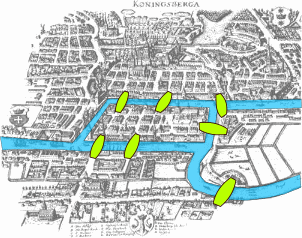
\includegraphics[width=0.48\textwidth]{bridges}
    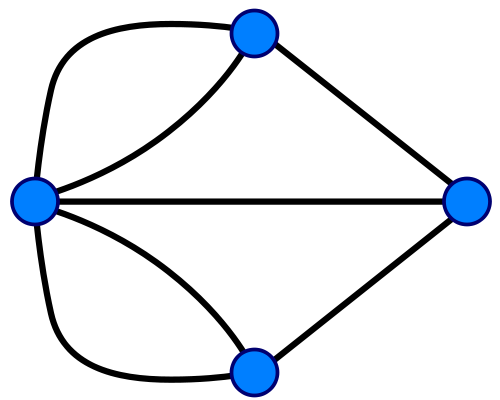
\includegraphics[width=0.48\textwidth]{bridges-graph}
  \end{figure}
  \begin{itemize}
    \item[] Can you walk cross every bridge only once?
      \pause
    \item[] It is \alert{impossible}, proved by Euler in 1735.
  \end{itemize}
\end{frame}

\subsection{Undirected Graphs}
\begin{frame}{Undirected Graphs}
  \begin{figure}
    \centering
    \includegraphics[width=\textwidth]{undirected}
  \end{figure}
  \begin{itemize}
    \item[] Simplified UK railway network.
    \item[] \alert{Nodes} represent cities and \alert{Edges} railway links.
  \end{itemize}
\end{frame}

\subsection{Directed graphs}
\begin{frame}{Directed Graphs}
  \begin{figure}
    \centering
    \includegraphics[width=\textwidth]{directed}
  \end{figure}
  \begin{itemize}
    \item[] My way from Glasgow to London.
    \item[] \alert{Edges} have a direction, because I am not interested in the
trains in the opposite direction.
  \end{itemize}
\end{frame}

\section{De Bruijn Graph}

\subsection{Permutations}

\begin{frame}{Permutations}
  \begin{itemize}
    \item[] Given an alphabet, say "\texttt{AGC}".
    \item[] All \alert{permutations} are:\\
\texttt{AAA, AAG, AAC, AGA, AGG, AGC, ACA, ACG, ACC \\
        GAA, GAG, GAC, GGA, GGG, GGC, GCA, GCG, GCC \\
        CAA, CAG, CAC, CGA, CGG, CGC, CCA, CCG, CCC }.
    \item[] Some of these sequences \alert{overlap} over part of the string,
e.g. \texttt{AGG} and \texttt{CGG} or \texttt{CGC} and \texttt{GGC}.
      \pause
    \item[] If we modify the size of the permuted sting to a value different
from the size of the alphabet, we can write \alert{overlaps} in the same way.
    \item[] For a string of length 5, we would find \texttt{AAAAC} and
\texttt{AAAAG} (among others).
  \end{itemize}
\end{frame}

\subsection{De Bruijn Graph}
\begin{frame}{De Bruijn Graph}{Example}
  De Bruijn graph for an alphabet "AB" and length of string 3.
  \begin{figure}
    \centering
    \includegraphics[width=0.6\textwidth]{deb}
  \end{figure}
\end{frame}

\begin{frame}{De Bruijn Graph}{How to build it}
  \begin{enumerate}
    \item To construct the de Bruijn graph on the previous slide we take the
string "ABA" (alphabet "AB" an length 3).
    \item We \alert{shift} all elements to the \alert{left} leaving "BA".
    \item For \alert{each letter} in the alphabet add it to the end of the
string, producing "BAA" and "BAB".
    \item Draw \alert{directed edges} from "ABA" to "BAA" and from "ABA" to "BAB".
    \item Repeat operation for "BAA" and "BAB".  Until no new edges can be
drawn.
  \end{enumerate}
\end{frame}

\subsection{Alignment}
\begin{frame}{Alignment}
  \begin{itemize}
    \item[] De Brujin graph is used for alignment because it is easy to
calculate a path through \alert{all} of its edges whilst walking each edge only
once (remember "Bridges of K{\"o}nigsberg").
    \item[] It is possible to walk the entire graph with a \alert{look ahead}
of the size of the alphabet.
    \item[] The graph has $ <\text{alphabet}^{\text{size of string}}> $ number
of nodes.
    \item[] The number of edges on the graph is slightly more complex.
    \item[] Without looking back lets try to draw the de Bruijn graph when the
alphabet is "AB" and the length of the string is 3.
  \end{itemize}
\end{frame}

\appendix

\begin{frame}{References}
\begin{thebibliography}{2}

\bibitem{rajaraman2013}
  Anand Rajaraman, Jure Leskovec and Jeffrey Ullman,
  \newblock \emph{Mining of Massive Datasets},
  \newblock Stanford University,
  2013.

\bibitem{rajaraman2013}
  Phillip Compeau, Pavel Pevzner and Glenn Tesler,
  \newblock \emph{How to apply de Bruijn graphs to genome assembly},
  \newblock Nature Biotechnology 29,
  2011.

\end{thebibliography}
\end{frame}

\end{document}

